% Define the type of document.
\documentclass[12pt, a4paper]{article}

% Set a more sensible document size.
\usepackage[margin=0.75in]{geometry}

% Set the language.
\usepackage[british]{babel}
    \usepackage{csquotes}

% Prevent words from being split accross lines.
\tolerance=1\emergencystretch=\maxdimen\hyphenpenalty=10000\hbadness=10000

% Allows images to be included.
\usepackage{graphicx}
    \graphicspath{ {./images/} }

% Allow the use of hyperlinks.
\usepackage[hidelinks]{hyperref}

% Allow disabling of floating objects.
\usepackage{float}

% Allow the use of listings.
\usepackage[T1]{fontenc}
\usepackage[dvipsnames]{xcolor}
\usepackage{listings}
    \lstset{
        language=C++,
        basicstyle=\linespread{1.3}\ttfamily,
        keywordstyle=[1]\color{Orchid},
        keywordstyle=[2]\color{Dandelion},
        keywordstyle=[3]\color{Cyan},
        keywordstyle=[4]\color{TealBlue},
        commentstyle=\color{Gray},
        tabsize=4,
        breaklines=true,
        captionpos=b,
        frame=single,
        escapechar=`,
        morekeywords=[2]{Eigen,JacobiSVD,MatrixXd,Matrix3d,Vector3d,Array3d,RowVector3d},
        morekeywords=[3]{transpose,row,singularValues,matrixU,matrixV,determinant,Identity,minCoeff,array},
        morekeywords=[4]{ComputeFullU,ComputeFullV,ComputeThinU,ComputeThinV},
    }

% Create some shortcut commands:
\newcommand{\highlight}[2]{\colorbox{#1}{\vphantom{Ay}#2}}
\newcommand{\removed}[1]{\highlight{pink}{#1}}
\newcommand{\added}[1]{\highlight{lime}{#1}}
\newcommand{\swapped}[2]{\removed{#1}\added{#2}}
\newcommand{\inline}[1]{\fbox{\texttt{#1}}}
\newcommand{\tab}[0]{\space\space\space\space}

% Sets the title.
\title{Computer Graphics: Geometry and Simulation\\Coursework 3: Debugging Geometry and Simulation}
\author{Oliver Jones (s2153980)}
\date{}

% Begin the document.
\begin{document}
\maketitle

\section*{}
    The code listings in this report highlight the changes made to the codebase.
    \removed{Pink} sections have been removed from the original code, while
    \added{green} ones have been added.

\section{As-Rigid-as-Possible Deformation}
    The bugs in this section were all found by simply running the code and
        observing the incorrect output.
    \autoref{fig:1} shows the progression of changes as the bugs are fixed.
    The leftmost image shows the original output, the second shows the output after
        the first bug is fixed, and so on.
    The rightmost image shows the final output after all bugs have been fixed.

    To find each bug, I carefully examined the code and compared it to the
        algorithm described in Lecture 15.
    This highlighted three bugs, the fixes for which can be seen in
        Listings~\ref{lst:a1} through~\ref{lst:c2}.
    To assess the correctness of these fixes, I ran the code again and observed the
        output.
    Once the output matched the expected output, I was confident that the bugs had
        been fixed.

    The changes shown in \autoref{lst:c2} include some optimisations which do not
        affect the behaviour of the code, while the bug fix itself is shown in
        \autoref{lst:c1}.

    \begin{figure}[H]
        \centering
        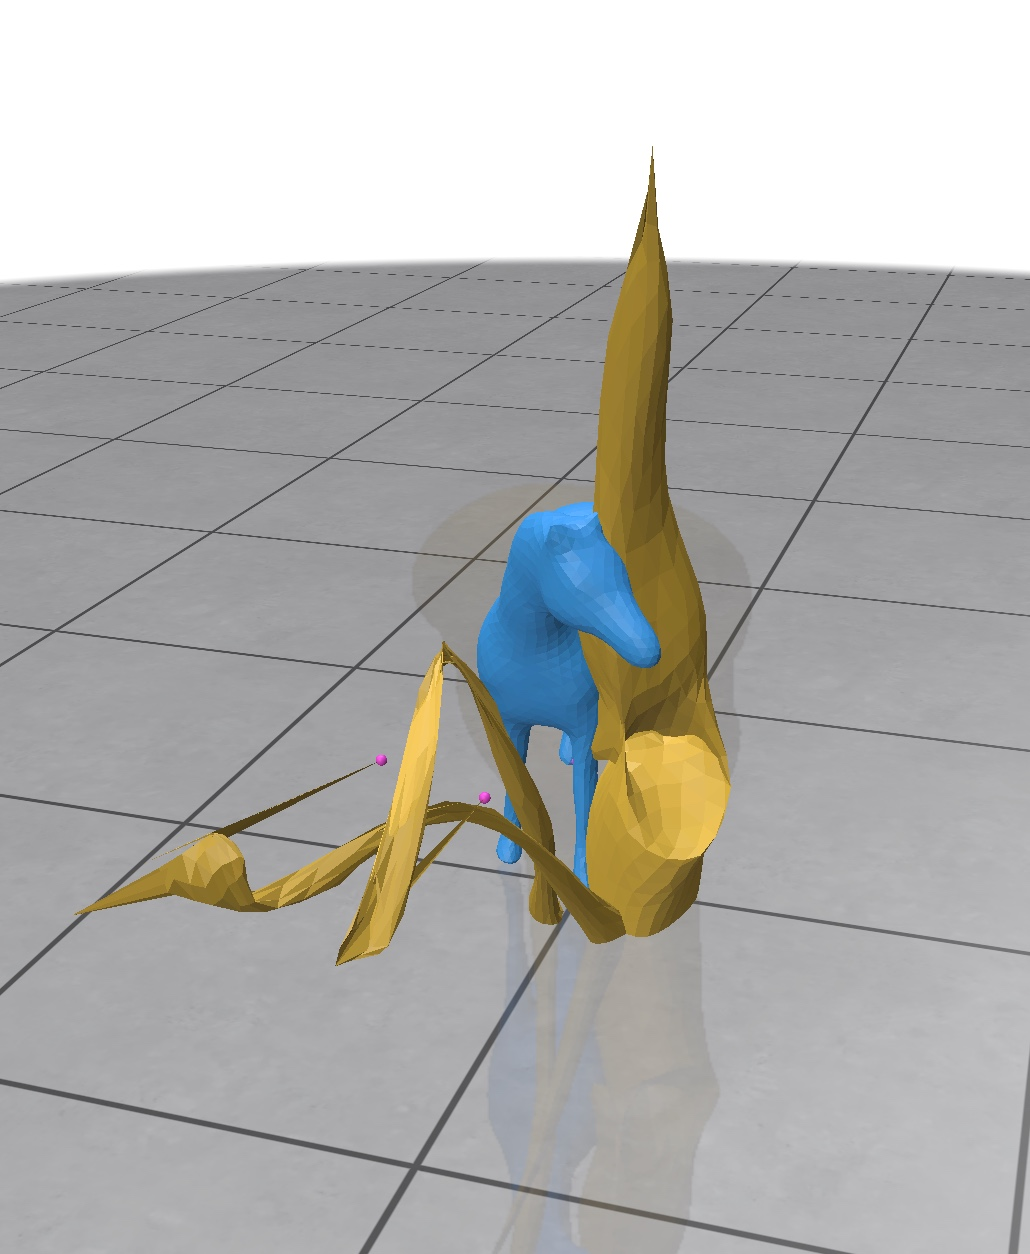
\includegraphics[width=0.2\textwidth]{images/1-0.png}
        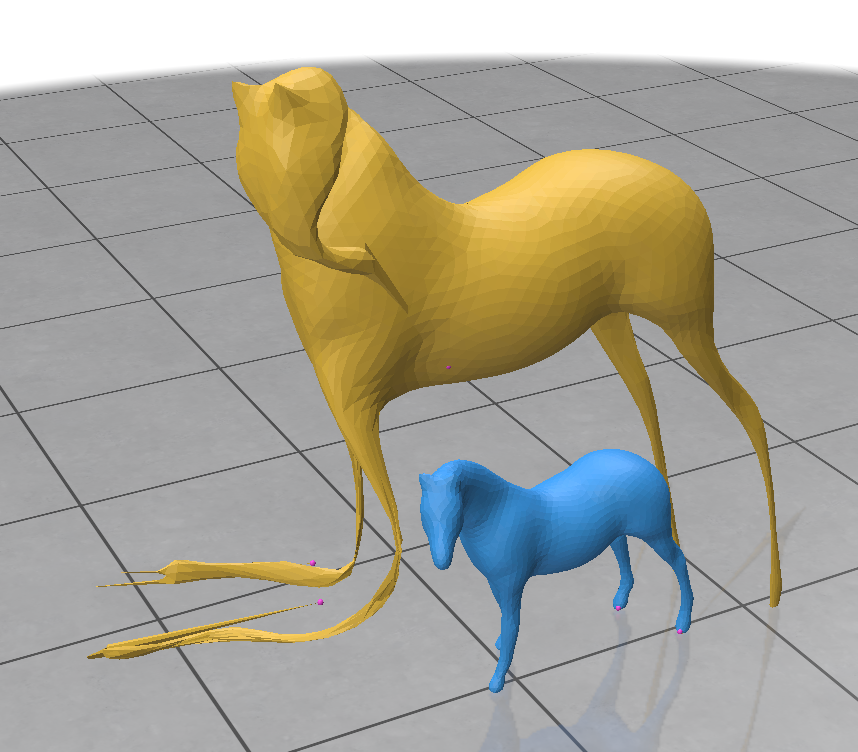
\includegraphics[width=0.2\textwidth]{images/1-1.png}
        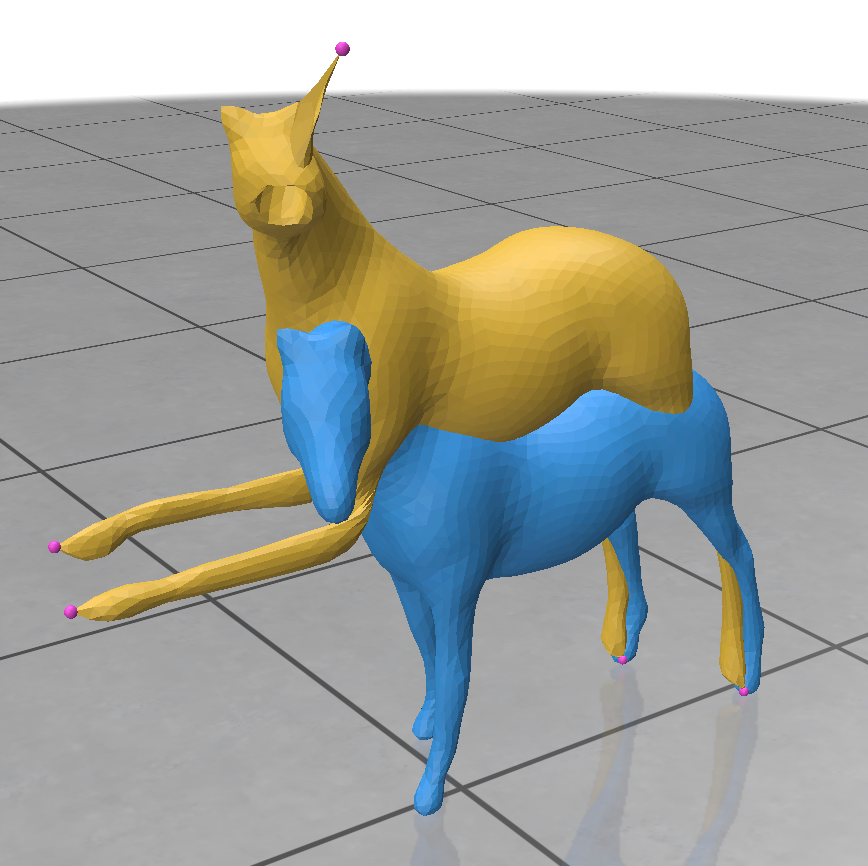
\includegraphics[width=0.2\textwidth]{images/1-2.png}
        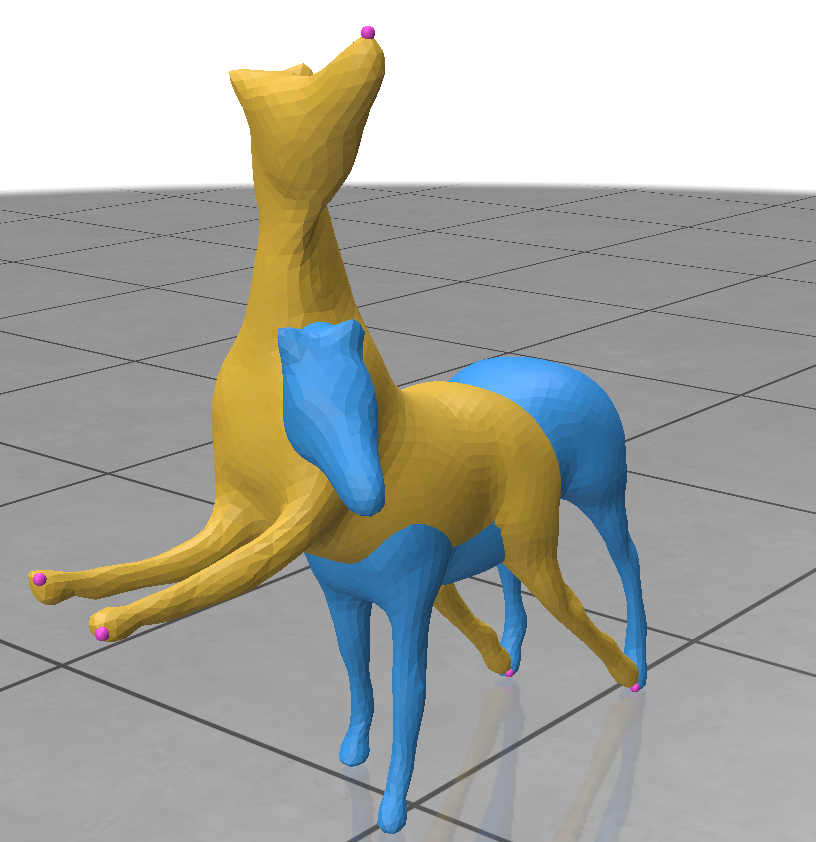
\includegraphics[width=0.2\textwidth]{images/1-3.png}
            % 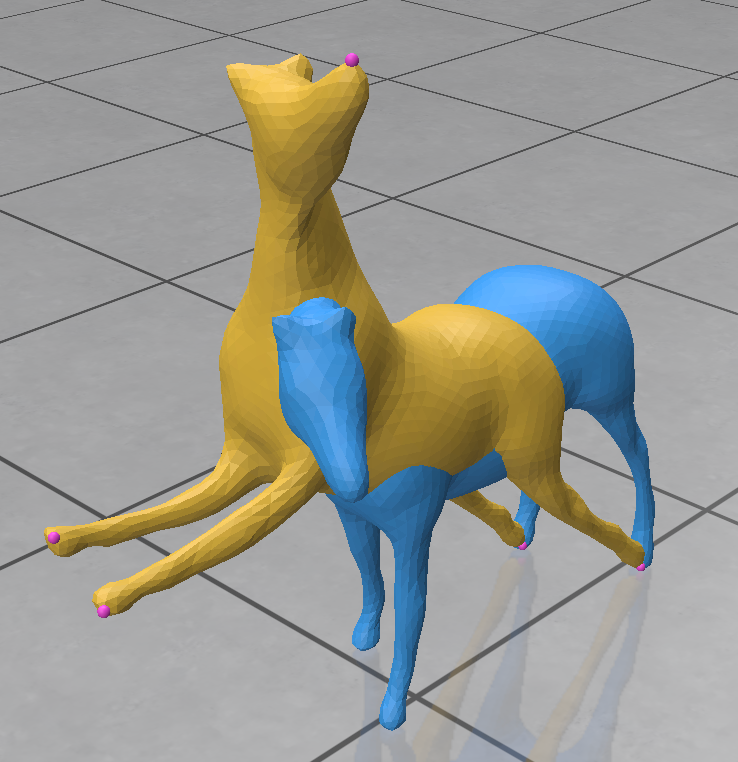
\includegraphics[width=0.2\textwidth]{images/1-4.png}
            \caption{The progression of changes as the bugs are fixed.}
            \label{fig:1}
    \end{figure}

    \subsection{Incorrect Rotation}
        \begin{lstlisting}[caption={The \inline{0} and \inline{1} have been swapped.}, label={lst:a1}]
g.row(j) = (origV.row(E(j, `\swapped{0}{1}`)) - origV.row(E(j, `\swapped{1}{0}`))) * REdge;
\end{lstlisting}

    \subsection{Missing W}
        \begin{lstlisting}[caption={The \inline{* W } was missing.}, label={lst:b1}]
MatrixXd rhs = d0I.transpose() `\added{* W }` * (g - d0B * constPositions);
\end{lstlisting}

    \subsection{Incorrect Multiplication}
        \begin{lstlisting}[caption={\inline{P} and \inline{Q} have been swapped.}, label={lst:c1}]
S = `\swapped{Q}{P}`.transpose() * `\swapped{P}{Q}`;
\end{lstlisting}

        \begin{lstlisting}[caption={Two redundant lines have been removed, and the \inline{for} loop has 
            been closed much earlier. The bug fix shown in \autoref{lst:c1} has also been applied.}, 
            label={lst:c2}]
for (int k = 0; k < oneRings[j].size(); k++) {
    P.row(k) = origV.row(oneRings[j][k]) - origV.row(j);
`\removed{\tab{}P.row(k) = origV.row(oneRings[j][k]) - origV.row(j);}`
    Q.row(k) = currV.row(oneRings[j][k]) - currV.row(j);
`\removed{\tab{}Q.row(k) = currV.row(oneRings[j][k]) - currV.row(j);}`
`\added{\}}`
`\removed{\tab}`S = `\swapped{Q}{P}`.transpose() * `\swapped{P}{Q}`;
// Several lines ommitted for brevity
`\removed{\tab}`R[j] = currR;
`\removed{\}}`
\end{lstlisting}

\section{Multi-body Rigid Simulation}
    The first bug in this section was found by running the code and observing the
        incorrect output.
    It was obvious that the forces between the spheres were reversed, and it was
        easy to find the bug by examining the code.
    Two possible fixes were identified, and are shown in Listings~\ref{lst:d1}
        and~\ref{lst:d2}.
    The next two bugs were less obvious in the output, but were found by carefully
        examining the code.

    The bug fix in \autoref{lst:e1} was a clear mathematical error.
    To check for a collision between two spheres, the distance between their
        centres must be less than the sum of their radii, i.e. $d<2r$.
    However, as this calculation is checking the square of the distance against the
        squares of the radii, the comparison should be $d^2<4r^2$, not $d^2<2r^2$.

    The final bug was a simple comparison error, as shown in \autoref{lst:f1}.
    To see the effect of this bug, I changed the value of \inline{CRCoeff} from
        \inline{0.0} to \inline{1.0}.
    This made it clear that the comparison was incorrect, as the spheres would not
        bounce when they hit the ground.

    \begin{figure}[H]
        \centering
        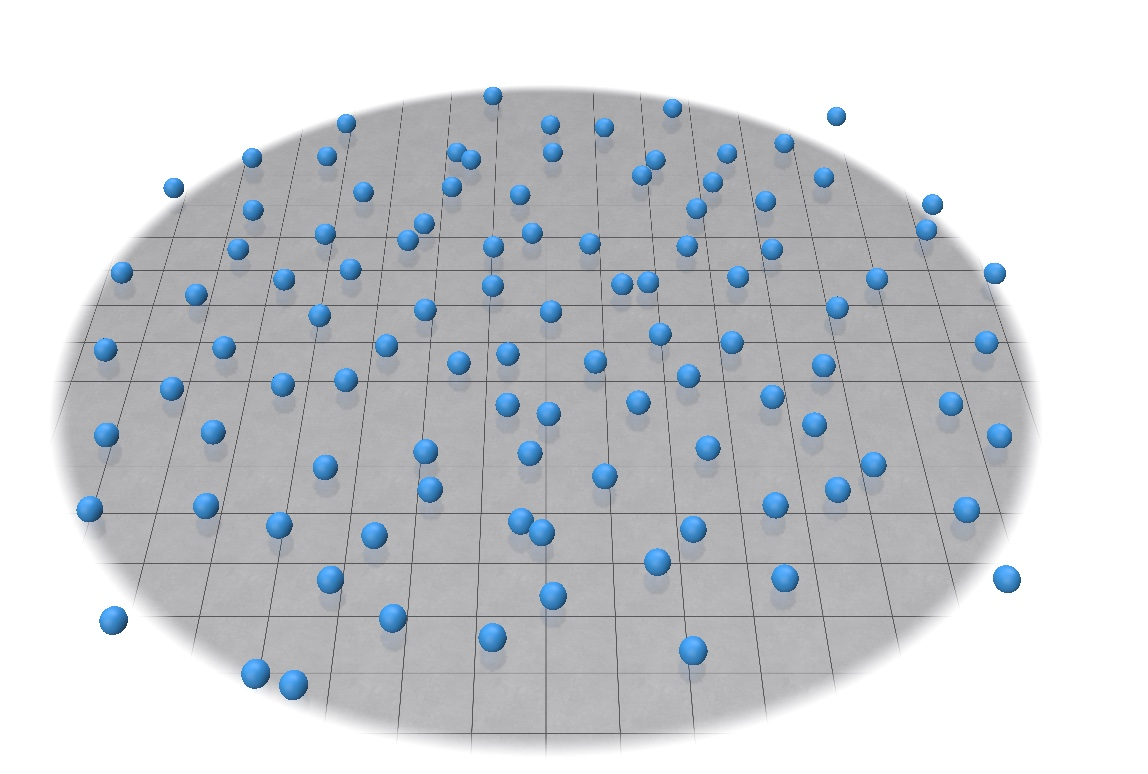
\includegraphics[width=0.2\textwidth]{images/2-0.png}
            % 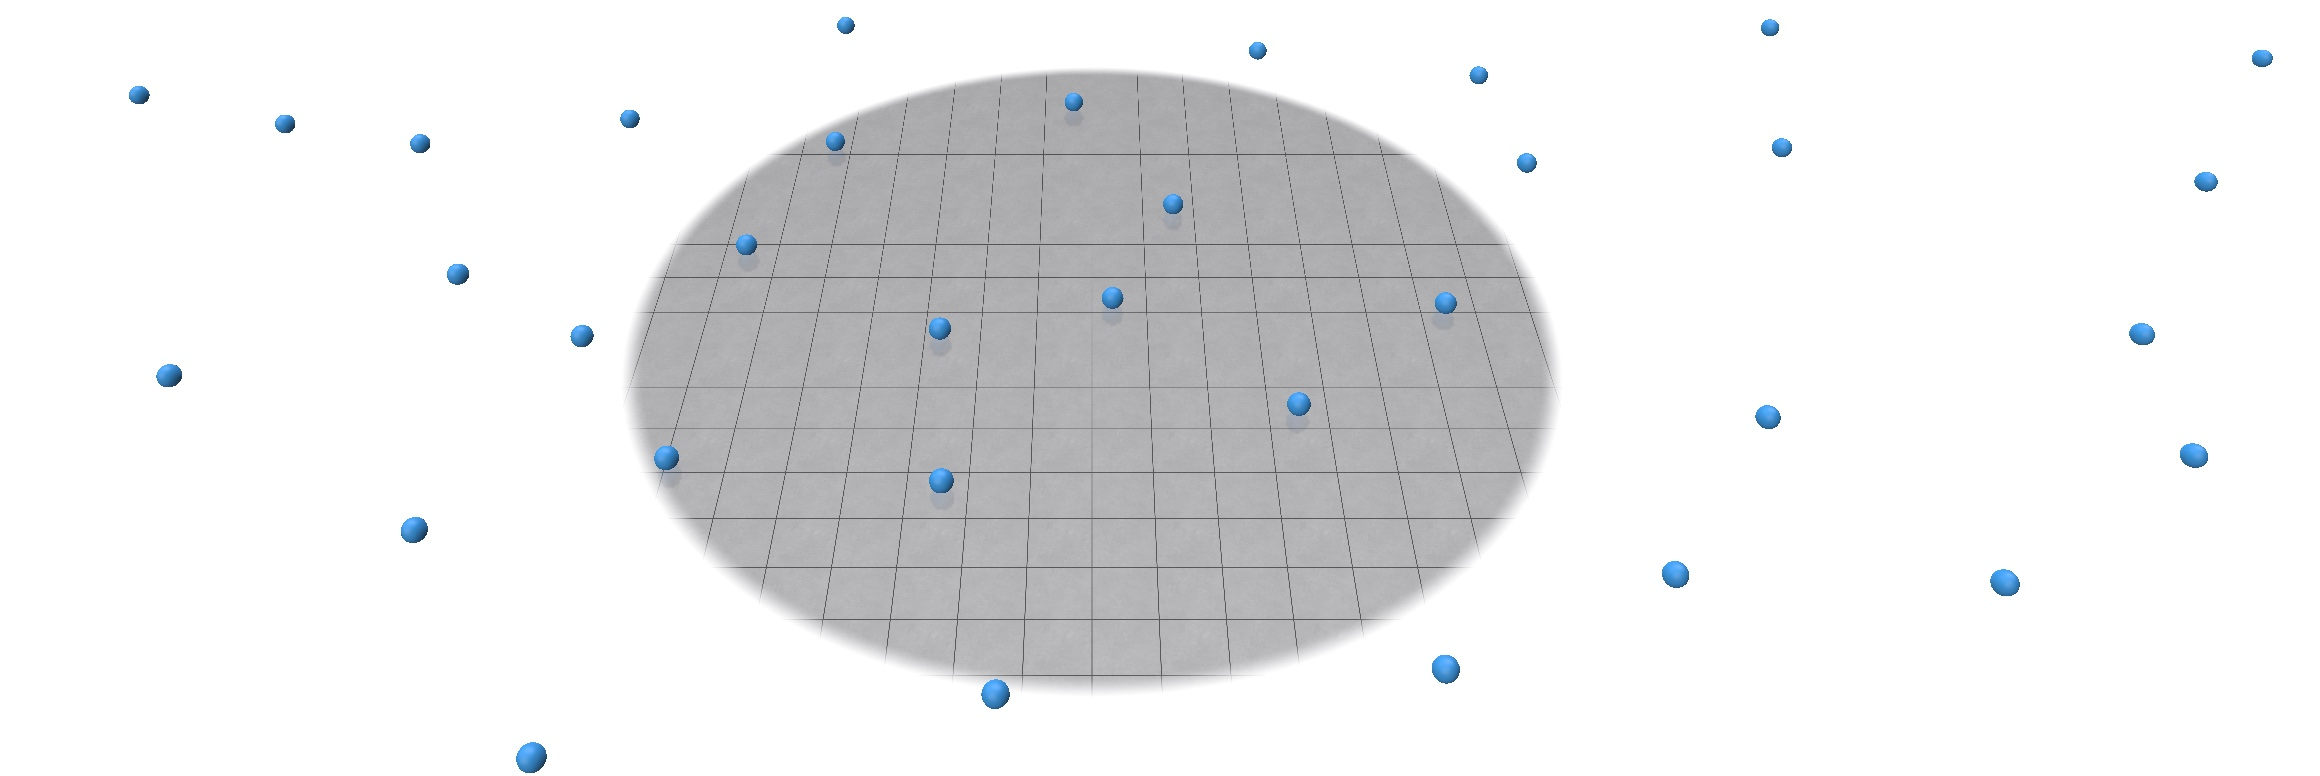
\includegraphics[width=0.2\textwidth]{images/2-1.png}
        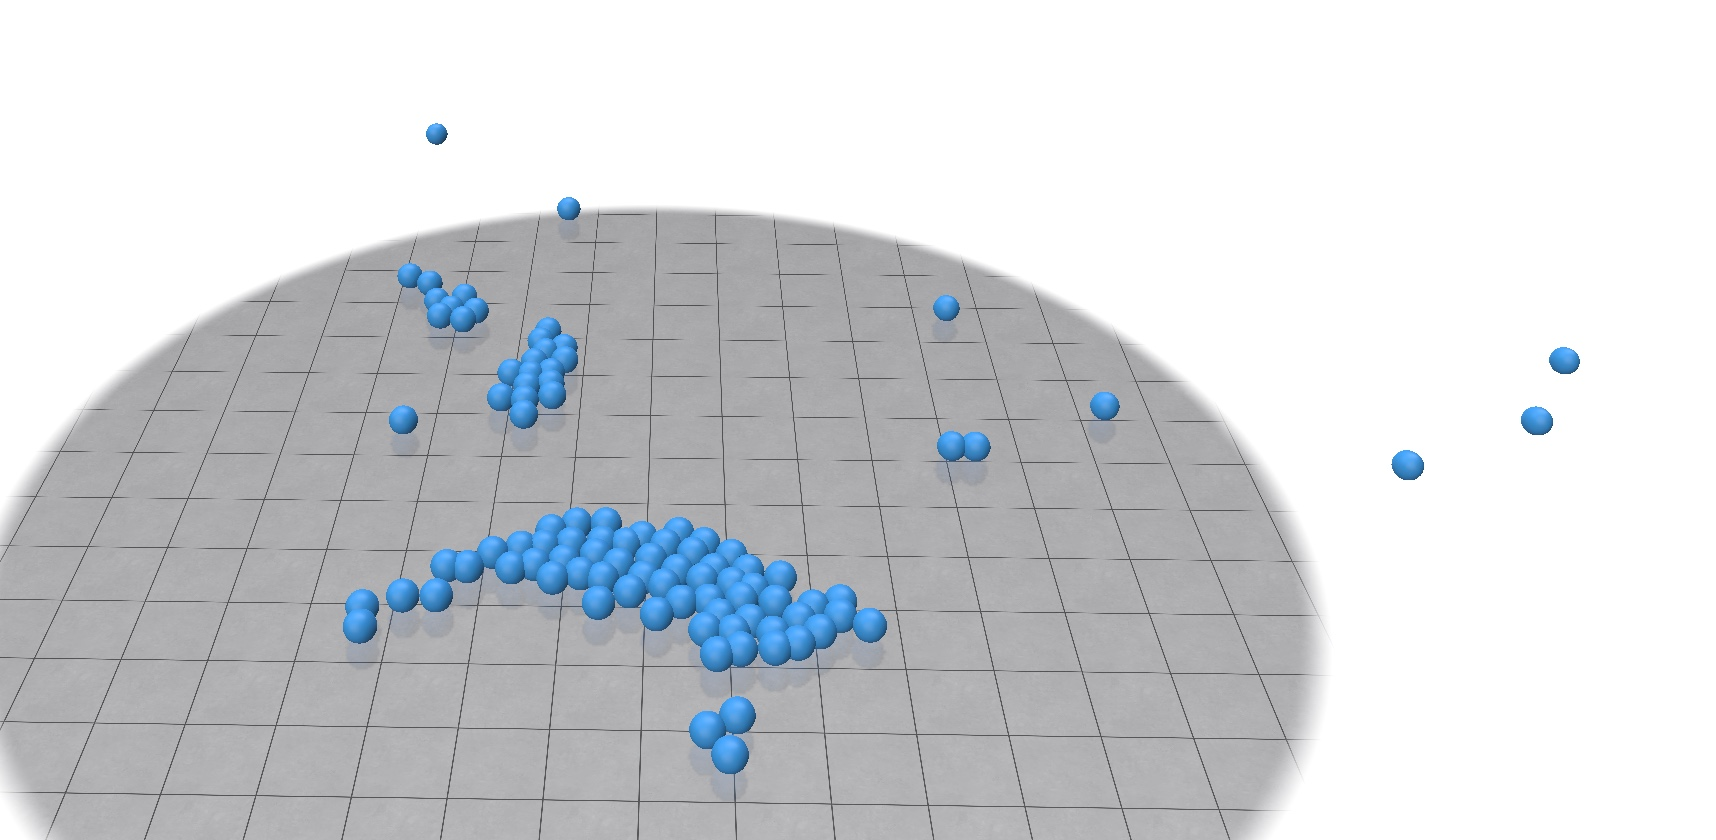
\includegraphics[width=0.2\textwidth]{images/2-2.png}
        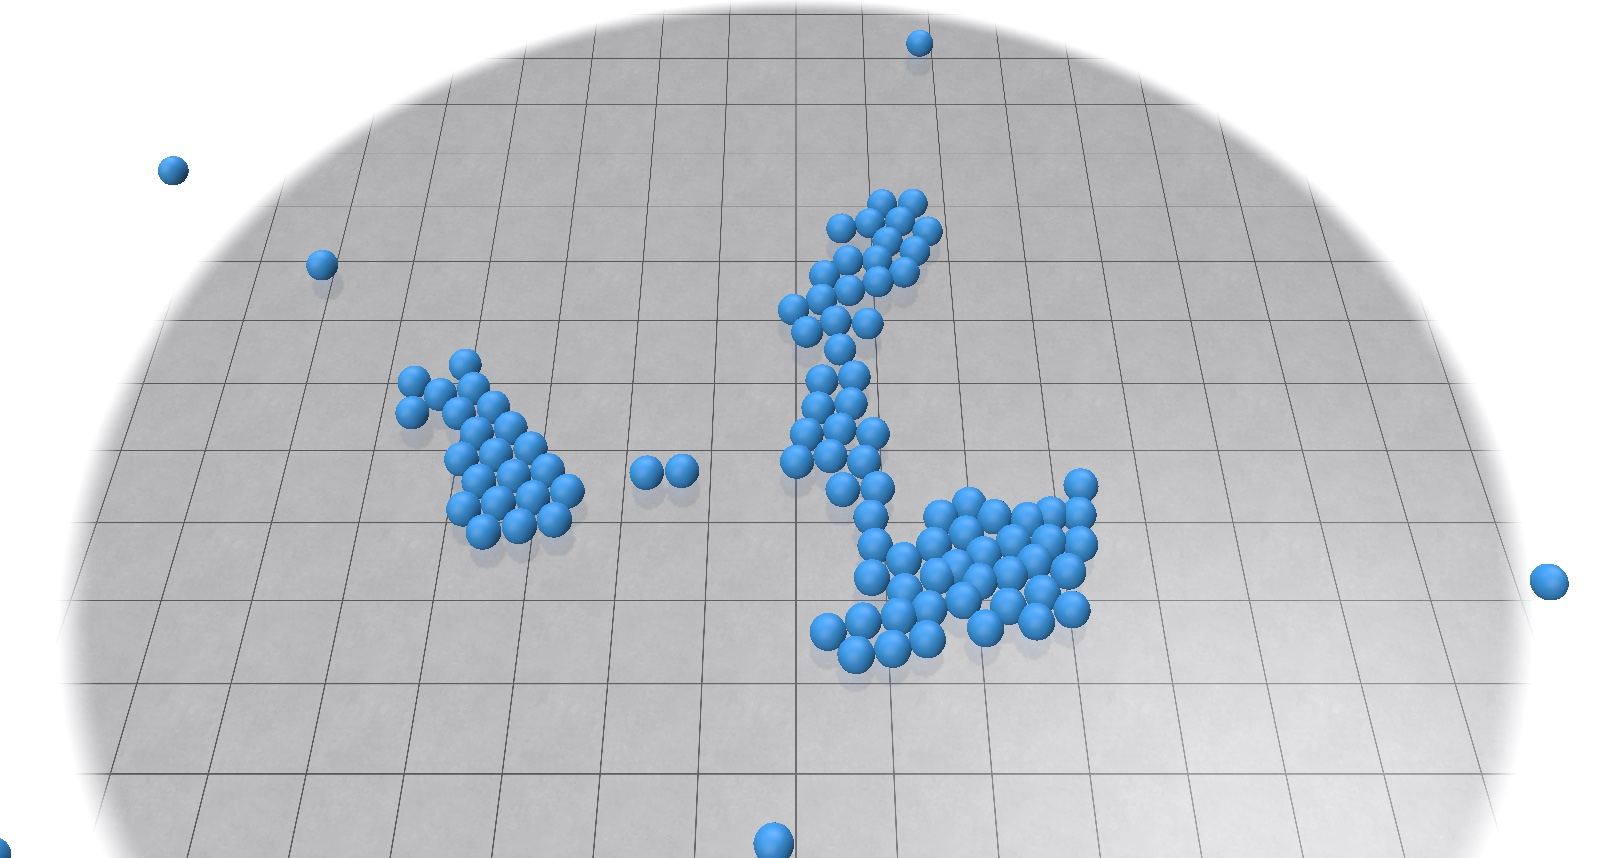
\includegraphics[width=0.2\textwidth]{images/2-3.png}
        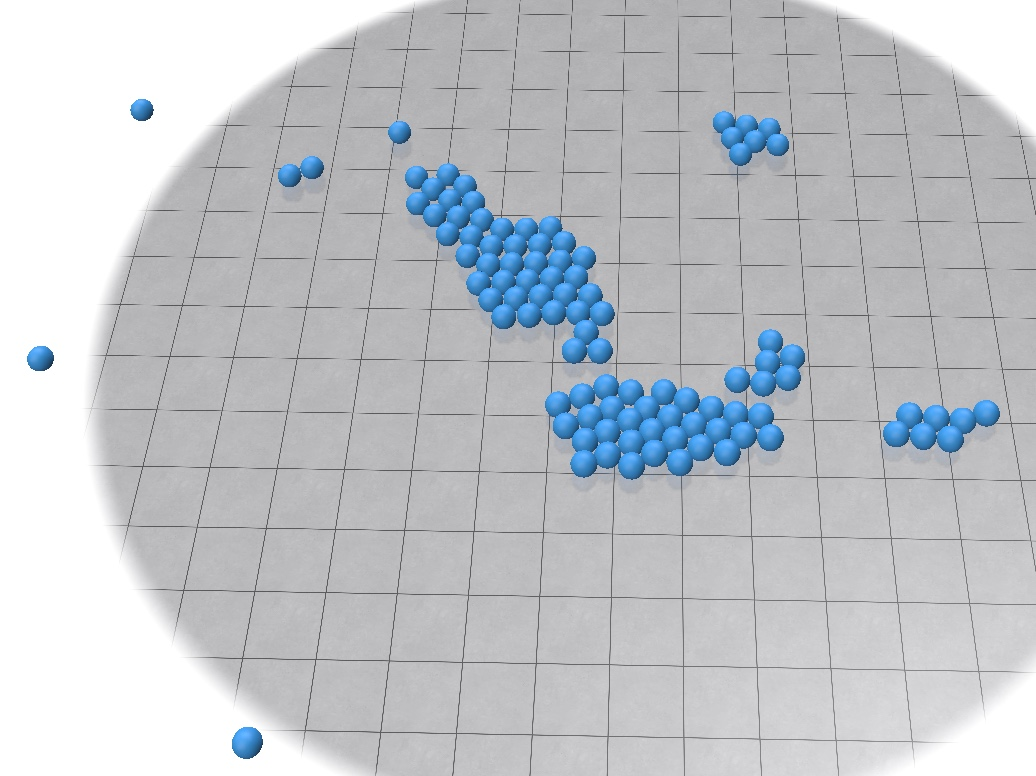
\includegraphics[width=0.2\textwidth]{images/2-4.png}
            \caption{The progression of changes as the bugs are fixed.}
            \label{fig:2}
    \end{figure}

    \subsection{Reversed Pairwise Gravity}
        \begin{lstlisting}[caption={The \inline{+} and \inline{-} have been swapped.}, label={lst:d1}]
forces.row(i).array() = forces.row(i) `\swapped{-}{+}` forceDirection * gravityConstant / sqrDistance;
forces.row(j).array() = forces.row(j) `\swapped{+}{-}` forceDirection * gravityConstant / sqrDistance;
\end{lstlisting}
        \begin{lstlisting}[caption={The \inline{i} and \inline{j} have been swapped.}, label={lst:d2}]
RowVector3d forceDirection = spherePoses.row(`\swapped{j}{i}`) - spherePoses.row(`\swapped{i}{j}`);
\end{lstlisting}

    \subsection{Incorrect Squared Radius Multiplier}
        \begin{lstlisting}[caption={The \inline{2} has been replaced with \inline{4}.}, label={lst:e1}]
if (sqrDistance < `\swapped{2}{4}` * sqrRadius)
\end{lstlisting}

    \subsection{Incorrect Zero Comparison}
        \begin{lstlisting}[caption={The \inline{>} has been swapped with \inline{<}.}, label={lst:f1}]
if (sphereVelocities(i, 1) `\swapped{>}{<}` 0.0)
\end{lstlisting}

\end{document}
